\documentclass{article}
\usepackage[utf8]{inputenc}
\usepackage{amsmath}
\usepackage{amssymb}
\usepackage{tikz}
\usepackage{setspace}

\title{Pythagorean Theorem}
\author{1505053 }
\date{\today}

\begin{document}

\maketitle


\section{Introduction}
In this document, we present the very famous theorem in mathematics: Pythagorean
theorem, which is stated as follows.


\textbf{Theorem 1.1 (Pythagorean theorem)} 
 \textit{The square of the hypotenuse (the
side opposite the right angle) is equal to the sum of the squares of the other two
sides.}
\par
Numerous mathematicians proposed various proofs to the theorem. The
theorem was long known even before the time of Pythagoras. Pythagoras was
the first to provide with a sound proof. The proof that Pythagoras gave was
by rearrangement. Even the great Albert Einstein also proved the theorem
without rearrangement, rather by using dissection. Figure 1 shows the visual
representation of the theorem.


\begin{tikzpicture}

\end{tikzpicture}

\begin{tikzpicture}[scale=0.4]

\draw [fill=cyan,cyan!10] (10,-6.5) --(10,10.2) -- (27.2,10.2) -- (27.2,-6.5) -- (10,-6.5);


%\draw (0,0) --(1,2) -- (2,3) -- (1,0) -- (-15,10);
\draw [fill =violet!60,violet!60] (17,0) --(20,0) -- (20,3) -- (17,3) -- (17,0);


\node [violet] at (18.8,2.7) {\large a};


\draw[fill=red!40,red!40](20,3) --(24,3) -- (24,7) -- (20,7) -- (20,3);

\node [violet] at (20.4,5) {\large b};


\draw [fill=cyan,cyan] (17,3) --(20,7) -- (16,10) -- (13,6) -- (17,3);

\node [violet] at (17.8,5) {\large c};


\draw [fill=cyan,cyan] (16,-1) --(11,-1) -- (11,-6) -- (16,-6) -- (16,-1);

\node at (16.8,-3.5) {\large{=}};

\draw [fill =violet!60,violet!60] (18,-2) --(21,-2) -- (21,-5) -- (18,-5) -- (18,-2);
\node at (22,-3.5) {\large{+}};

\draw[fill=red!40,red!40](23,-1.5) --(27,-1.5) -- (27,-5.5) -- (23,-5.5) -- (23,-1.5);


\draw[red!60,line width=0.7](17,3) --(20,7) -- (20,3) -- (17,3);

\draw[cyan,line width=0.7](19.5,3) --(19.5,3.5) -- (20,3.5) ;




\node [violet] at (12.5,-3.5) {\large $c^2$};

 \node [violet] at (4.5,-3.5) {\large .};

\node [violet] at (25.5,-3.5) {\large $b^2$};
\node [violet]  at (19,-3.5){$a^2$}
\end{tikzpicture}

\begin{center}
    Figure 1: Visual representation of the famous Pythagorean theorem
\end{center}


\newpage

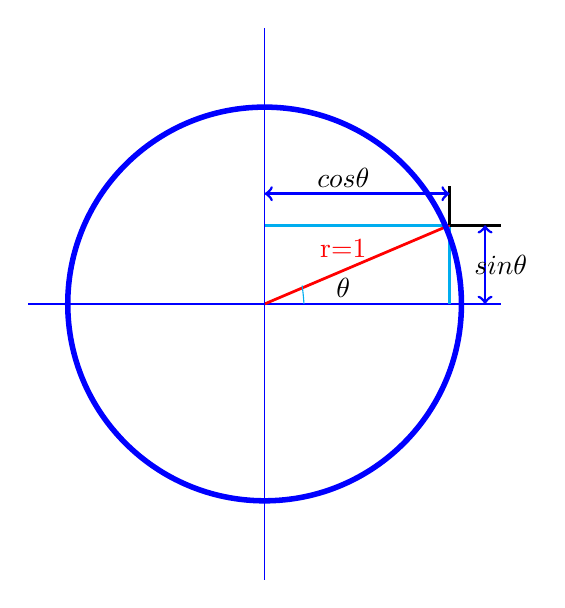
\begin{tikzpicture}



\draw[blue,line width=0.5](12,0) --(18,0) ;



\draw[cyan,line width=1](15,1) --(17.35,1) ;

\draw[cyan,line width=1](17.35,1)--(17.35,0) ;

\draw[red,line width=1](15,0) --(17.35,1) ;


\draw[blue,line width=0.5](15,3.5) --(15,-3.5)  ;

\draw[black,line width=1](17.35,1)--(18,1) ;
\draw[black,line width=1](17.35,1)--(17.35,1.5) ;

\draw[blue,line width=1,<->](15,1.4)--(17.35,1.4) ;

\draw[blue,line width=1,<->](17.8,1)--(17.8,0) ;


\draw [blue,line width=2] (15,0) circle [radius=2.5];;




\node [black] at (16,1.6) { $cos \theta $};

\node [black] at (18,0.5) { $ sin \theta $};

\node [red] at (16,.7) { r=1};

 \draw[cyan] (15.5,0) arc (3.5:8:3);

\node [black] at (16,.2) {$ \theta $};


%\draw[very thick] (0,0) to [out=0,in=5] (5,7);



\end{tikzpicture}

\begin{center}
  
  Figure 2: Alternate representation of Pythagorean theorem
\end{center}


\section{Trigonometric Forms}
Lots of other forms of the same theorem exist. The most useful, perhaps, are
expressed in trigonometric terms, as follows:
\par 
\par
\begin{equation}
\\
    sin^2\theta + cos^2 \theta =1  
\end{equation}
\begin{equation}
    sec^2\theta - tan^2 \theta =1   
\end{equation}
\begin{equation}
\\
cosec^2 \theta -cot^2 \theta =1
\end{equation}

\subsection{Representing the First}

Taking 1, we can show them as shown in Figure2. When we take a point at
unit distance from the origin, the y and x co-ordinates become sin θ and cos θ
respectively. Therefore, sum of the squares of the two becomes equal to the
square of the unit distance, which of course, is 1.
    
    









\end{document}